\documentclass[11pt]{beamer}
\usetheme{Rochester}
\usepackage{amsmath} %основной пакет для формул
\usepackage[utf8]{inputenc}
\usepackage[english,russian]{babel}
\usepackage[OT1]{fontenc}
\usepackage{amsfonts}
\usepackage{amssymb}
\usepackage{here}
\usepackage{hyperref}
\beamertemplatenavigationsymbolsempty
\author{Дьячков Вадим Вадимович\\
Жуйков Артём Александрович\\
Ламтев Антон Юрьевич\\
Леженин Юрий Игоревич\\}
\title[Методы сжатия изображений]{Методы сжатия изображений}
\setbeamercovered{transparent} 
%\setbeamertemplate{navigation symbols}{} 
%\logo{} 
\institute{Санкт-Петербургский политехнический университет Петра Великого\\
Институт компьютерных наук и технологий\\
Кафедра компьютерных систем и программных технологий\\
Группа 13501/4} 
\date{\the\year}
\begin{document}


\begin{frame}
\titlepage
\end{frame}


%\begin{frame}{Актуальность темы}
%\begin{itemize}
%	\item повседневное использование людьми сжатых изображений
%	\item 
%\end{itemize}
%\end{frame}


\begin{frame}{Методы сжатия}
\begin{itemize}
	\item Цветовое пространство $YC_bC_r$ и цветовая субдискретизация
	\item Квантование и дискретизация
	\item Вейвлет сжатие
	\item Алгоритм RLE
	\item Алгоритм LZW
	\item Алгоритм Хаффмана
	%\item \dots
\end{itemize}
\end{frame}



\begin{frame}{Цветовое пространство $YC_bC_r$ и цветовая субдискретизация}
\begin{block}{Цветное изображение и его компоненты Y, $C_B$ и $C_R$}
\begin{figure}[H]
	\begin{center}
		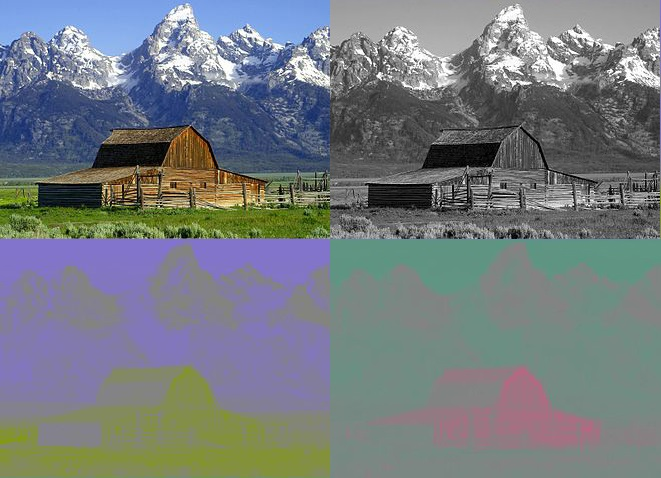
\includegraphics[scale=0.77]{../pics/YCbCr/YCbCr_separation_vert.jpg}
	\end{center}
	%\center{Цветное изображение и его компоненты Y, $C_B$ и $C_R$}
\end{figure}
\end{block}
\end{frame}



\begin{frame}{Цветовое пространство $YC_bC_r$ и цветовая субдискретизация}
\begin{block}{Плоскость $YC_bC_r$ при постоянной яркости Y = 0.5}
\begin{figure}[H]
	\begin{center}
		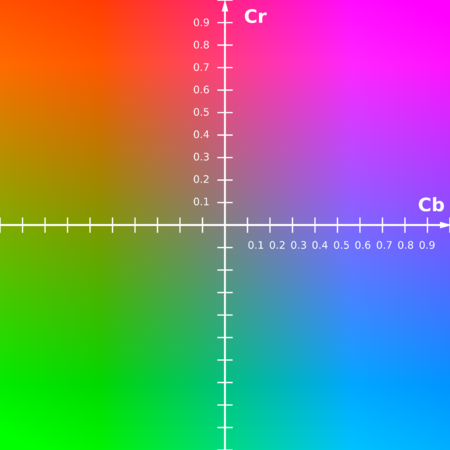
\includegraphics[scale=0.5]{../pics/YCbCr/YCbCr.png}
	\end{center}
	%\center{Плоскость $YC_bC_r$ при постоянной яркости Y = 0.5}
\end{figure}	
\end{block}			
\end{frame}



\begin{frame}{Цветовое пространство $YC_bC_r$ и цветовая субдискретизация}
\begin{block}{Форматы субдискретизации}
\begin{figure}[H]
	\begin{center}
		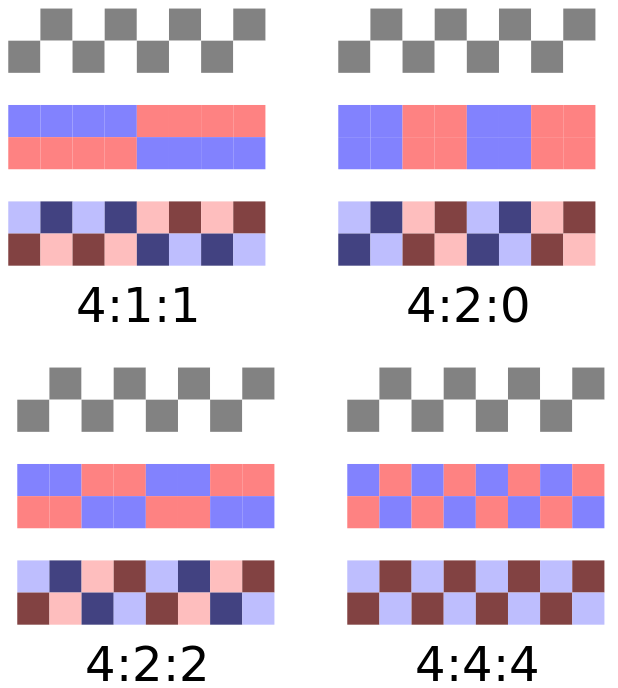
\includegraphics[scale=0.38]{../pics/chroma_subsampling/chroma_subsampling_ratios_pr.png}
		%\center{Форматы субдискретизации}
	\end{center}
\end{figure}	
\end{block}				
\end{frame}



\begin{frame}{Квантование и дискретизация}
\begin{block}{Уменьшение точности дискретизации}
\begin{figure}[H]
	\begin{center}
		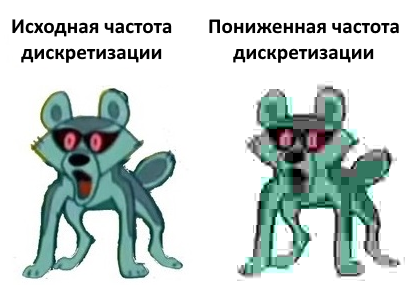
\includegraphics[scale=0.73]{../pics/quantization/shakal.png}
		%\caption{Уменьшение точности дискретизации} 
	\end{center}
\end{figure}	
\end{block}				
\end{frame}



\begin{frame}{Квантование и дискретизация}
\begin{block}{Уменьшение точности квантования}
\begin{figure}[H]
	\begin{center}
		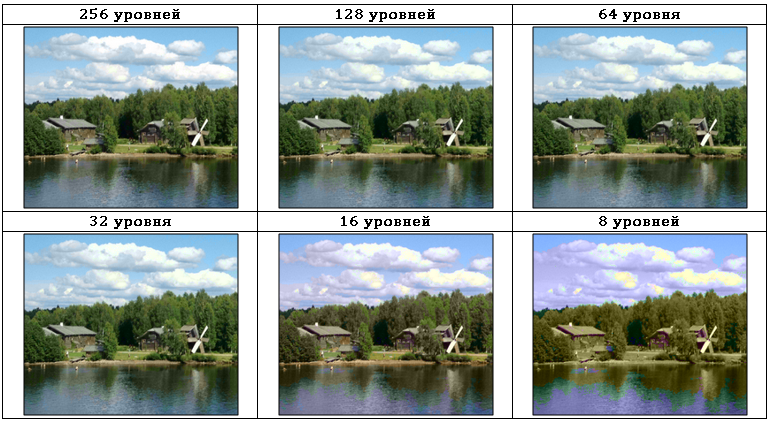
\includegraphics[scale=0.5]{../pics/quantization/levels_of_quantization.png}
		%\caption{Уменьшение точности квантования} 
	\end{center}
\end{figure}	
\end{block}				
\end{frame}



\begin{frame}{Вейвлет сжатие}
\begin{block}{Одномерное преобразование Хаара}
\begin{figure}[H]
	\begin{center}
		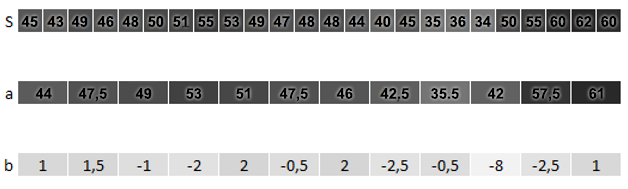
\includegraphics[scale=0.65]{../pics/wavelet/example.png}
		%\caption{Пример для одномерного пространства} 
	\end{center}
\end{figure}	
\end{block}				
\end{frame}



\begin{frame}{Вейвлет сжатие}
\begin{block}{Двумерное преобразование Хаара. Сжатие}
\begin{figure}[H]
	\begin{center}
		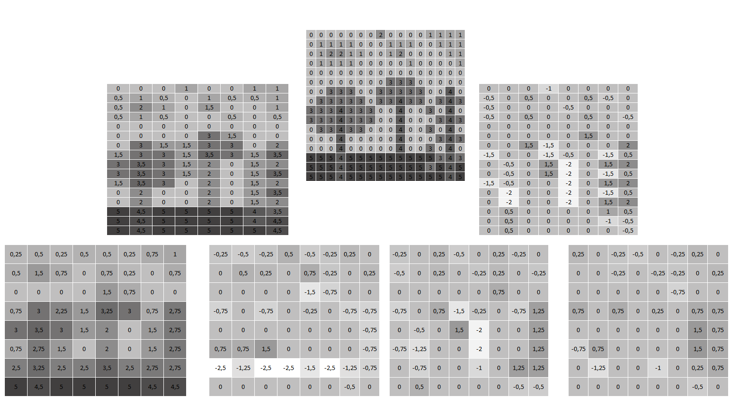
\includegraphics[scale=0.53]{../pics/wavelet/compression_pr.png}
		%\caption{Процесс сжатия} 
	\end{center}
\end{figure}	
\end{block}				
\end{frame}



\begin{frame}{Вейвлет сжатие}
\begin{block}{Двумерное преобразование Хаара. Восстановление}
\begin{figure}[H]
	\begin{center}
		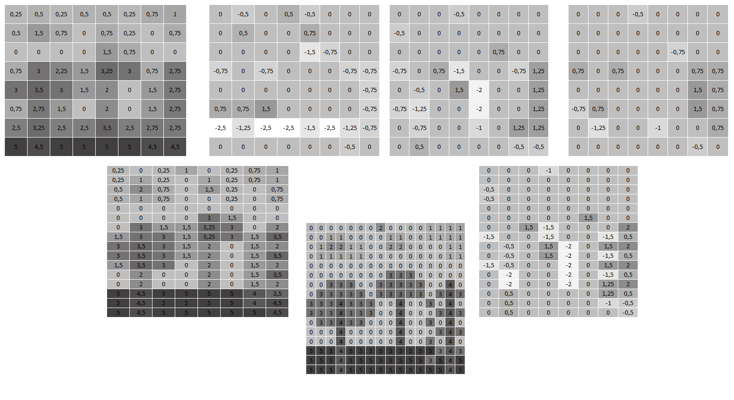
\includegraphics[scale=0.53]{../pics/wavelet/uncompression_pr.png}
		%\caption{Процесс восстановления} 
	\end{center}
\end{figure}	
\end{block}				
\end{frame}



\begin{frame}{Алгоритм LZW}
\begin{block}{Начальный словарь}
\begin{figure}[H]
	\begin{center}
		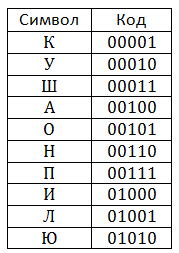
\includegraphics[scale=0.8]{../pics/LZW/dictionary.png}
		%\caption{Начальный словарь}
	\end{center}
\end{figure}	
\end{block}				
\end{frame}


 
\begin{frame}{Алгоритм LZW}
\begin{block}{Процесс и результат кодирования}
\begin{figure}[H]
	\begin{center}
		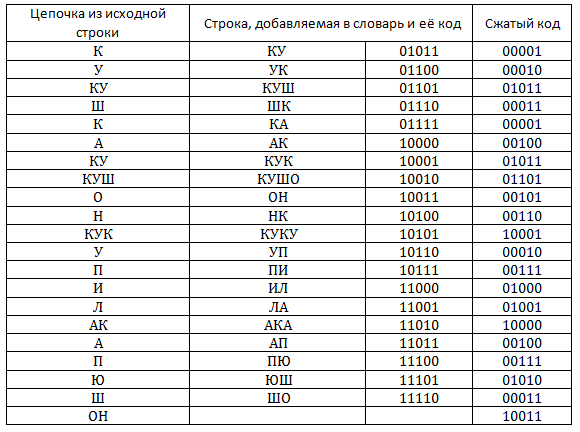
\includegraphics[scale=0.55]{../pics/LZW/result.png}
		%\caption{Процесс и результат кодирования}
	\end{center}
\end{figure}	
\end{block}				
\end{frame} 
 


\begin{frame}{Алгоритм RLE}
\begin{block}{Процесс и результат кодирования}
\begin{figure}[H]
	\begin{center}
		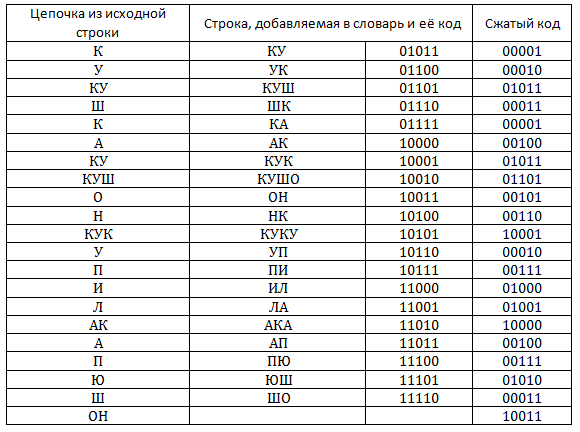
\includegraphics[scale=0.55]{../pics/LZW/result.png}
		%\caption{Процесс и результат кодирования}
	\end{center}
\end{figure}	
\end{block}				
\end{frame} 


\begin{frame}{Дискретное косинусное преобразование}
\begin{block}{Комбинация горизонтальных и вертикальных частот}
\begin{figure}[H]
	\begin{center}
		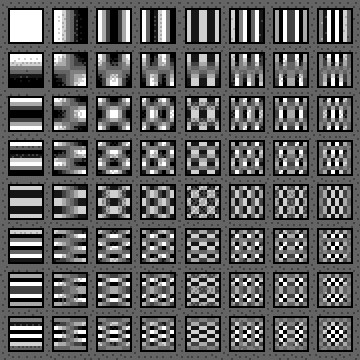
\includegraphics[scale=0.35]{../pics/cosine_transform/matrix.png}
		%\caption{Процесс и результат кодирования}
	\end{center}
\end{figure}	
\end{block}				
\end{frame} 


\begin{frame}{Сжимаем аудиторию}
\begin{figure}[H]
	\begin{center}
		\huge\href{http://octo.ejiek.com/job/image_compression_algorithms/}{магия}
	\end{center}
\end{figure}					
\end{frame} 



\begin{frame}{}
\begin{center}
	\huge Спасибо за внимание!!!
	
\includegraphics[scale=0.5]{../pics/smile.jpg}
\end{center}				
\end{frame}

\end{document}
